%%%%%%%%%%%%%%%%%%%%%%%%%%%%%%%%%%%%%%%%%%%%%%%%%%%%%%%%%
% 
%%%%%%%%%%%%%%%%%%%%%%%%%%%%%%%%%%%%%%%%%%%%%%%%%%%%%%%%%%

\chapter{\babTiga}
Perancangan serta langkah-langkah di perlukan untuk menyelesaikan penelitian ini. Berikut ini akan di jelaskan gambaran serta tahapan dari perancangan system yang di teliti serta skenario simulasi dari hasil desain yang telah dirancang.

%%%%%%%%%%%%%%%%%%%%%%%%%%%%%%%%%%%%%%%%%%%%%%%%%%%%%%%%%%
% 
%%%%%%%%%%%%%%%%%%%%%%%%%%%%%%%%%%%%%%%%%%%%%%%%%%%%%%%%%%

\section{Perancangan Desain}

Desain utama adalah desain modul alu. Pada penelitian kali ini digunakan modul ALU dengan 2 register masing-masing 8 bit \textit{input}, 4 bit \textit{opcode} dan 8 bit \textit{output} seperti ditunjukan pada diagram dibawah ini.

\begin{figure}
	\centering
	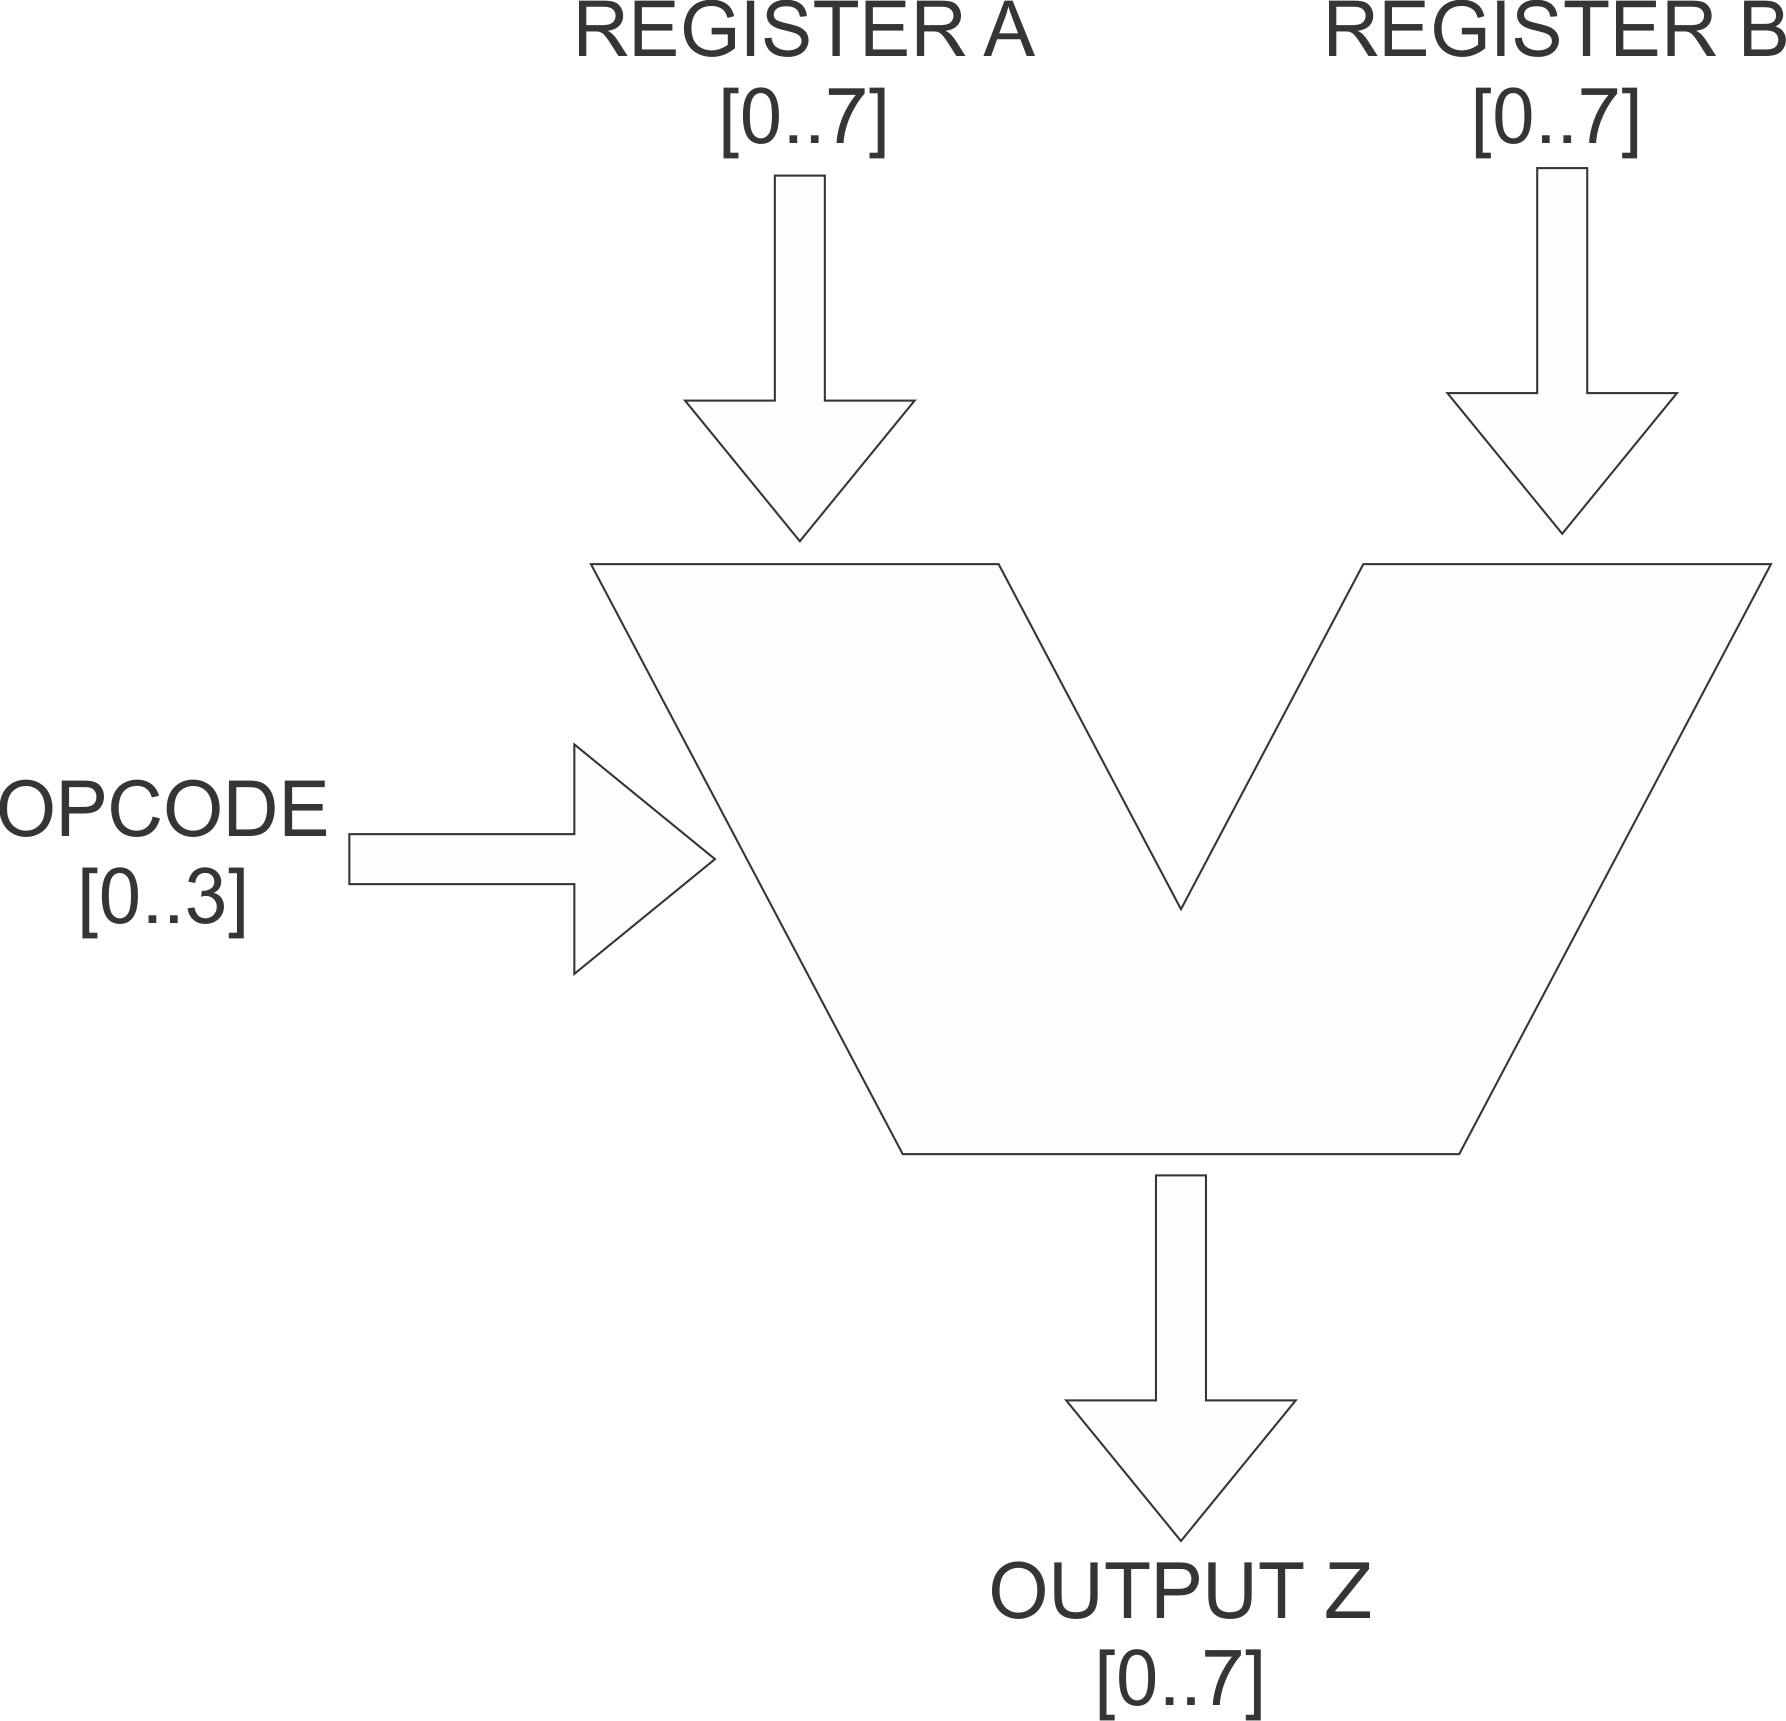
\includegraphics[width=0.5\textwidth]
	{ilustrasi/aludesain.png}
	\caption{Desain ALU yang akan dilindungi}
	\label{aludesain}
\end{figure}

Selain menggunakan desain ALU penulis juga merancang desain perlindungan dengan input 4 bit dan output 8 bit seperti yang ditunjukan diagram dibawah ini. modul inilah yang nantinya akan diselipkan pada modul ALU.

\begin{figure}
	\centering
	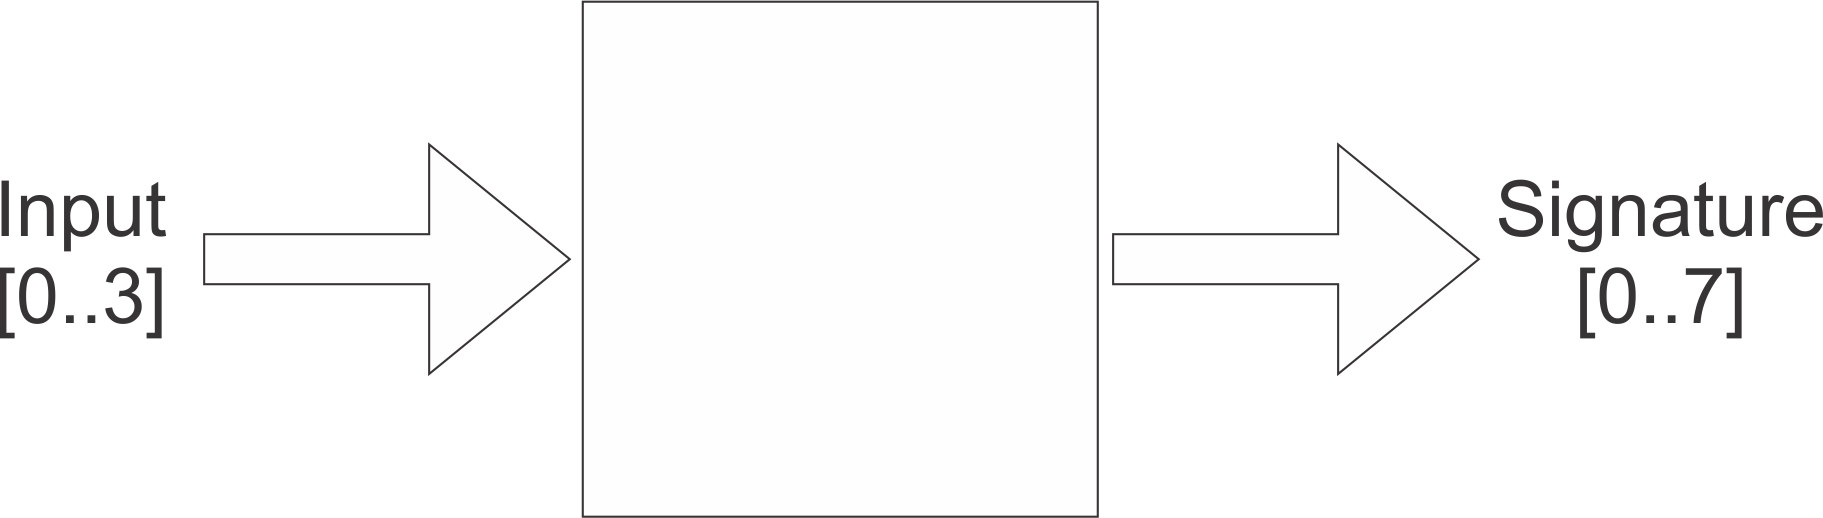
\includegraphics[width=0.5\textwidth]
	{ilustrasi/watermarkdesain.png}
	\caption{Desain rangkaian pelindung}
	\label{watermarkdesain}
\end{figure}

\subsection{Skema Perlindungan}

Skema perlindungan ini dilakukan teknik Pengolahan Sinyal Digital untuk ekstraksi data \textit{signature} dan \textit{obfuscation} dengan \textit{polymorph gate} untuk menyembunyikan keberadaan \textit{signature}. Dibawah berikut merupakan spesifikasi I/O pada modul yang akan dilindngi.

\begin{figure}
	\centering
	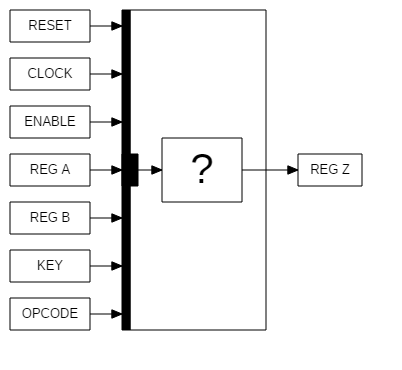
\includegraphics[width=0.5\textwidth]
	{diagrams/topAsk.png}
	\caption{Desain rangkaian Top modul yang terdapat rangkaian lain}
	\label{topAsk}
\end{figure}

Untuk teknik \textit{obfuscation} dengan \textit{polymorph} dilakukan desain yang bertujuan menyelipkan suatu modul lain pada modul utama tanpa diketahui pengguna. Teknik ini seperti memberikan program \textit{Trojan} kedalam suatu program utama. Namun sub-program ini bukan untuk merusak namun untuk melindungi. Seperti ilustrasi di atas menunjukan suatu modul besar namun ada sesuatu lain di dalam modul tersebut.

\begin{figure}
	\centering
	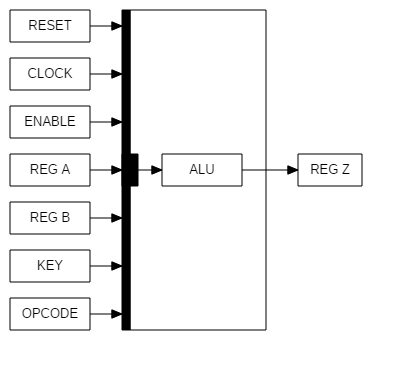
\includegraphics[width=0.5\textwidth]
	{diagrams/topAlu.png}
	\caption{Desain rangkaian ALU pada top modul}
	\label{topAlu}
\end{figure}

Pertama dengan menggunakan rangkaian ALU sebagai modul besar (utama) dengan spesifikasi I/O \textit{chip} yang telah ditentukan sebelumnya. Lalu fungsional ALU ditest dengan spesifikasi yang telah dibuat. 

\begin{figure}
	\centering
	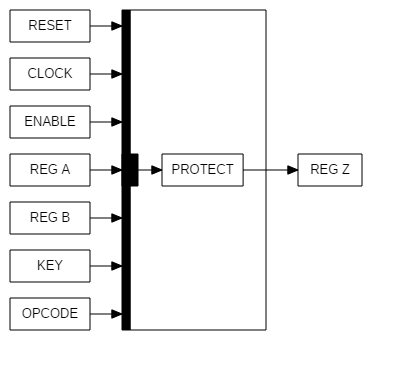
\includegraphics[width=0.5\textwidth]
	{diagrams/topPro.png}
	\caption{Desain rangkaian pelindung pada top modul}
	\label{topPro}
\end{figure}

Setelah itu ganti rangkaian modul ALU dengan modul perlindungan sebagai modul utama kemudian dilakukan tes fungsional kembali untuk mengetahui apakah rangkaian perlindungan dapat bekerja diatas arsitektur serta spesifikasi modul utama.

Setelah didapat kedua modul dapat berjalan sesuai dengan semestinya maka langkah selanjutnya menggabungkan kedua modul tersebut bada modul utama. pada penggabungan kali ini digunakan teknik \textit{obfuscation polymorph} untuk memilih antara modul mana yang harus berjalan pada modul utama.

\begin{figure}
	\centering
	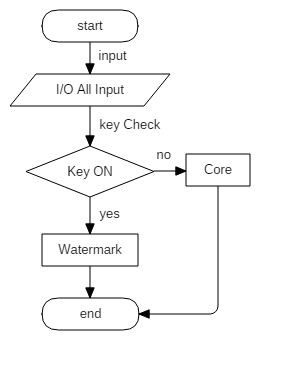
\includegraphics[width=0.5\textwidth]
	{diagrams/Activation.png}
	\caption{Algoritma aktifasi}
	\label{fig:aktifasi}
\end{figure}

Diagram diatas menunjukan bagaimana cara mengaktifkan modul dengan key sebagai kontroler. Untuk hasil \textit{output} diperlukan kontrol tambahan penjembatan antara hasil \textit{output} modul ALU dan modul perlindungan seperti pada ilustrasi di bawah agar tidak terjadi bentrokan antara kedua output,

\begin{figure}
	\centering
	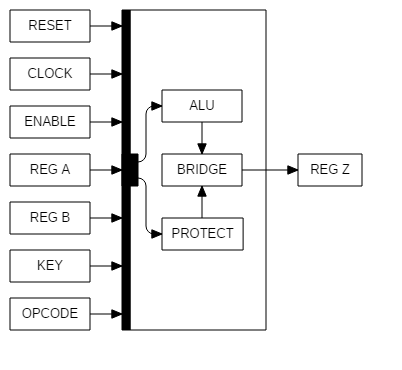
\includegraphics[width=0.5\textwidth]
	{diagrams/top.png}
	\caption{Desain rangkaian top modul yang telah diberi pelindung}
	\label{top}
\end{figure}

dibawah ini merupakan contoh listing program pada ilustrasi di atas. Sehingga terdapat 1 Top modul dan 3 sub modul pada desain chip yang telah diberikan rangkaian pelindung.\\\\

\begin{lstlisting}[language=Verilog]
// Main Modul IC Watermark
module alu( RST, CLK, ENA, RGA, RGB, RGZ, KEY, OPT);
    // Deklarasi I/O
    input  RST, CLK, ENA;
    input  [3:0]OPT;
    input  [7:0]RGA,RGB;
    input  [1:0]KEY;
    output [7:0]RGZ;
    wire   [7:0]A,B,RGZ;
    // Core Inti
    alu_min aluj(RST, CLK, ENA, RGA, RGB, A, KEY, OPT);
    // Protektor
    protection prot(RST, CLK, ENA, RGA, RGB, B, KEY);
    // Bridge antara core dan protektor
    bridge jembatan(A, B, RGZ);
endmodule
\end{lstlisting}

Listing program merupakan representasi dari desain pada \textbf{lampiran 5}.

\subsection{Spesifikasi}
Spesifikasi rangkaian dapat dilihat di \textbf{lampiran A1 dan A2} serta untuk desain RTL rangkaian perlindungan dapat dilihat pada \textbf{lampiran C2 }.

%%%%%%%%%%%%%%%%%%%%%%%%%%%%%%%%%%%%%%%%%%%%%%%%%%%%%%%%%%
% 
%%%%%%%%%%%%%%%%%%%%%%%%%%%%%%%%%%%%%%%%%%%%%%%%%%%%%%%%%%

\section{Alur Proses Pengembangan}
Secara garis besar pada sisi desainer, terdapat 3 langkah untuk melakukan pengembangan alat dari \textit{programming} hingga layout siap cetak. Penulis menggunakan cara ini dari hasil studi serta eksperimen saat proses pengembangan alat.

\begin{figure}
	\centering
	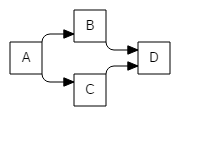
\includegraphics[width=0.3\textwidth]{diagrams/All_General.png}
	\caption{Skema Perancangan Umum Proses Desain}
\end{figure}

Pada langkah pertama dilakukan proses A, penulis melakukan perancangan desain dari IC yang akan di watermark kemudian di lakukan analisis. Apabila pertama telah selesai, penulis akan melakukan langkah kedua. Pada langkah kedua ini di lakukan kegiatan B yaitu proses ferifikasi dengan FPGA dan kegiatan C yaitu proses syntesys menjadi \textit{Raw Layout}. Setelah kegiatan B dan C selesai maka kegiatan D yaitu proses finalisasi layout dapat dilakukan yang akhirnya hasil final layout dapat di serahkan ke pabrik untuk di fabrikasi.

\begin{figure}
	\centering
	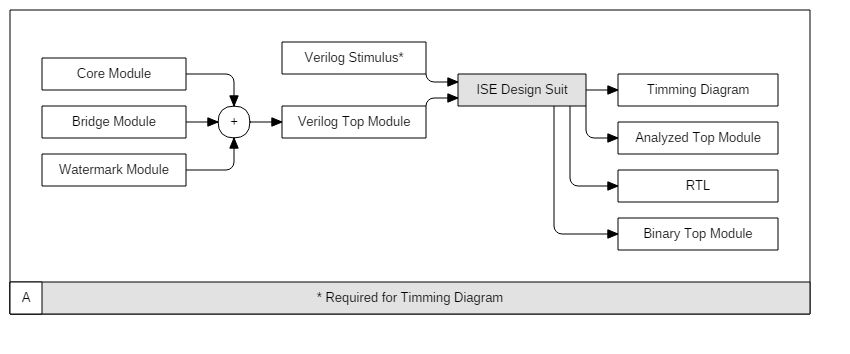
\includegraphics[width=1.0\textwidth]
	{diagrams/kegiatanA.png}
	\caption{Skema kegiatan A}
	\label{kegiatanA}
\end{figure}

Secara umum pada kegiatan A, penulis membuat 3 module \textit{verilog} untuk digabungkan. \textit{Core Module} yaitu program rangkaian ALU, Watermark Modul adalah program untuk watermarking dan Bridge Module untuk menghubungkan output antara \textit{Core Module} dan Watermark Modul. Setelah selesai dilakukan programming setiap medule tersebut maka medul-modul tadi digabungkan menjadi Top Module. \textit{Top Module} ini lah yang nantinya akan menjadi IC ter-watermark. 

Pada top module ini harus diberikan program tambahan yaitu stimulus untuk dapat mensimulasikan skenario Input dan \textit{Output} dari \textit{Top Module}. Bila sekenario stimulus telah dibuat, kemudian dilakukan simulasi dengan bantuan \textit{softwere ISE} design suit untuk melihat hasil simulasi berupa \textit{Timming diagram}. Pada \textit{Timming Diagram} inilah dapat di lihat apakah sekenario dari Input dan Output sesuai dengan keinginan. Setelah hasil analisis sesuai dengan yang diinginkan maka dilanjutkan dengan kegiatan selanjutnya yaitu kegiatan B dan C.

\begin{figure}
	\centering
	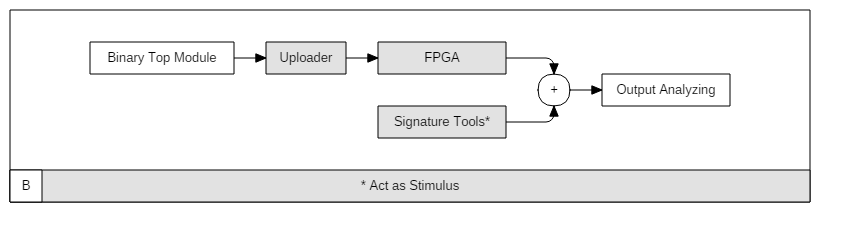
\includegraphics[width=1.0\textwidth]
	{diagrams/kegiatanB.png}
	\caption{Skema kegiatan B}
	\label{kegiatanB}
\end{figure}

Pada kegiatan B ini dilakukan simulasi ferivikasi pada \textit{board FPGA} dengan alat ferifikasi. kegiatan ini dilakukan untuk simulasi ferifikasi signature pada IC yang telah diwatermark. IC yang telah diwatermak di tanam pada FPGA dan dengan menggunakan \textit{Signature Tools} dilakukan ferifikasi sehingga didapat data \textit{signature} dari IC yang telah di watermask.

\begin{figure}
	\centering
	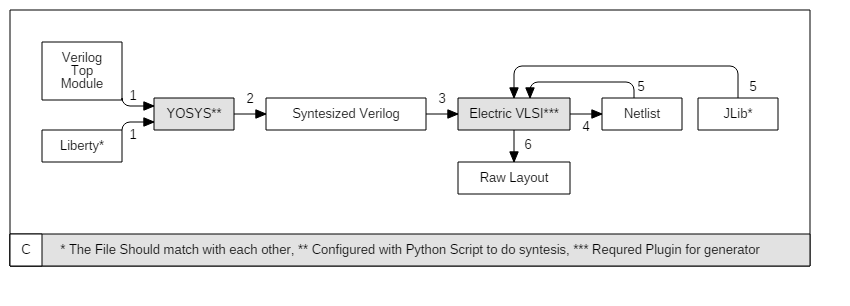
\includegraphics[width=1.0\textwidth]
	{diagrams/kegiatanC.png}
	\caption{Skema kegiatan C}
	\label{kegiatanC}
\end{figure}

Untuk kegiatan C dilakukan developing layout dari Top Module yang telah diferifikasi dengan \textit{timming diagram}. Defeloping menggunakan softwere Electric VLSI. Dengan men-\textit{synthesis} \textit{Verilog Top Module} dan \textit{Liberty} file menggunakan \textit{YOSYS}, maka akan di dapat file verilog tersyntesis. Kemudian File tersintesis tersebut di Load di Electric VLSI untuk di rubah ke \textit{NetList}. Setelah berhasil di rubah menjadi \textit{NetList} maka file NetList tersebut di kompilasi bersama file \textit{JLib} pada electric VLSI untuk di jadikan \textit{Raw Layout}.

\begin{figure}
	\centering
	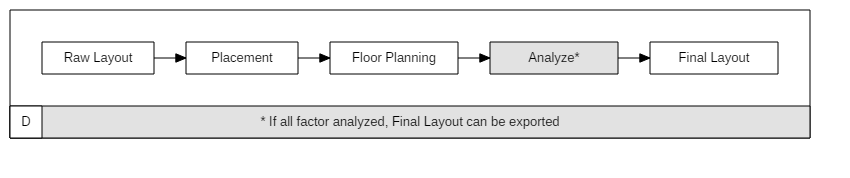
\includegraphics[width=1.0\textwidth]
	{diagrams/kegiatanD.png}
	\caption{Skema kegiatan D}
	\label{kegiatanD}
\end{figure}

Pada tahap ini di lakukan kegiatan C yaitu memproses \textit{Raw Layout} menjadi Final Layout yang siap di cetak. Tahapan nya adalah melakukan placement untuk setiap modulnya lalu di lakukan analisis kemudian dilakukan Floor planning. Setelah itu dilakukan analisis kembali hingga didapat hasil yang terbaik. Apabila telah didapat hasil yang terbaik maka File siap untuk difabrikasi.

%%%%%%%%%%%%%%%%%%%%%%%%%%%%%%%%%%%%%%%%%%%%%%%%%%%%%%%%%%
% 
%%%%%%%%%%%%%%%%%%%%%%%%%%%%%%%%%%%%%%%%%%%%%%%%%%%%%%%%%%

\section{Simulasi}
Simulasi dilakukan pada 2 environment, yaitu simulasi softwere (Timming diagram) serta simulasi hardwere (FPGA). Simulasi Timming diagram menggunakan simulator multisim yang tersedia sebagai fitur dari ISE Design Suit. Fitur ini bisa digunakan dengan langsung menjalankan simulator pada Top modul dan memasukan sinyal yang akan ditest atau menggunakan kode tambahan sebagai testbench. Keuntungan menggunakan tesbench ini kita bisa mengatur skenario simulasi pada top modul dan mempermudah dalam melakukan uji perangkat bila banyak sinyal dan faktor yang perlu di uji.

\begin{figure}
	\centering
	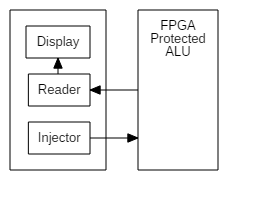
\includegraphics[width=0.5\textwidth]
	{diagrams/SimulasiAlat.png}
	\caption{Simulasi Alat}
	\label{SimulasiAlat}
\end{figure}
